% Máquina de estados implícita de rp_bram_sm (osciloscopio stock de Red Pitaya).
% El RTL no tiene un case(state): el estado vive en el par (adc_we, adc_dly_do).
% Fuente: rtl/classic/rp_bram_sm.v — documentado en
% docs/osc/sistema_adquisicion_original.md §3
%
% Compilar:   pdflatex fsm_rp_bram_sm.tex
% Incluir:    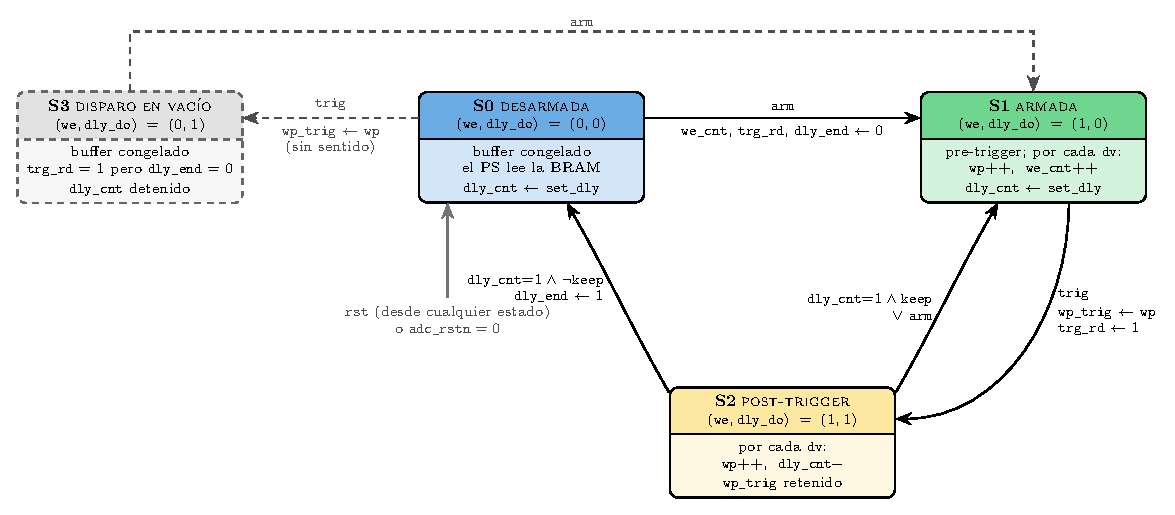
\includegraphics[width=\textwidth]{fsm_rp_bram_sm.pdf}
%
\documentclass[border=0pt,tikz]{standalone}
\usepackage[utf8]{inputenc}
\usepackage[T1]{fontenc}
\usepackage{lmodern}
\usepackage{amsmath}
\usetikzlibrary{arrows.meta,positioning,calc,shapes.multipart,quotes,backgrounds}

% ---------------------------------------------------------------- colores ---
\definecolor{azul}{RGB}{108,172,228}
\definecolor{verde}{RGB}{110,214,142}
\definecolor{amarillo}{RGB}{252,232,160}
\definecolor{grisr}{RGB}{226,226,226}

% ---------------------------------------------------------------- estilos ---
\tikzset{
  >={Stealth[length=2.6mm,width=2mm]},
  estado/.style = {
    rectangle split, rectangle split parts=2, rounded corners=4pt,
    draw=black, line width=0.7pt, align=center, text width=3.6cm,
    inner sep=3pt, font=\footnotesize,
    rectangle split part fill={#1, #1!30},
  },
  anomalo/.style = {estado=grisr, dashed, draw=black!60},
  trans/.style   = {->, line width=0.8pt},
  global/.style  = {->, line width=0.8pt, black!55},
  guarda/.style  = {font=\scriptsize, align=center, fill=white, inner sep=1.5pt},
}

% nombres de señales
\newcommand{\s}[1]{\texttt{#1}}
% encabezado de estado: nombre y codificación (adc_we, adc_dly_do)
\newcommand{\cab}[3]{\textbf{#1}\;\textsc{#2}\\[-1pt]{\scriptsize$(\s{we},\s{dly\_do}) = (#3)$}}

\begin{document}
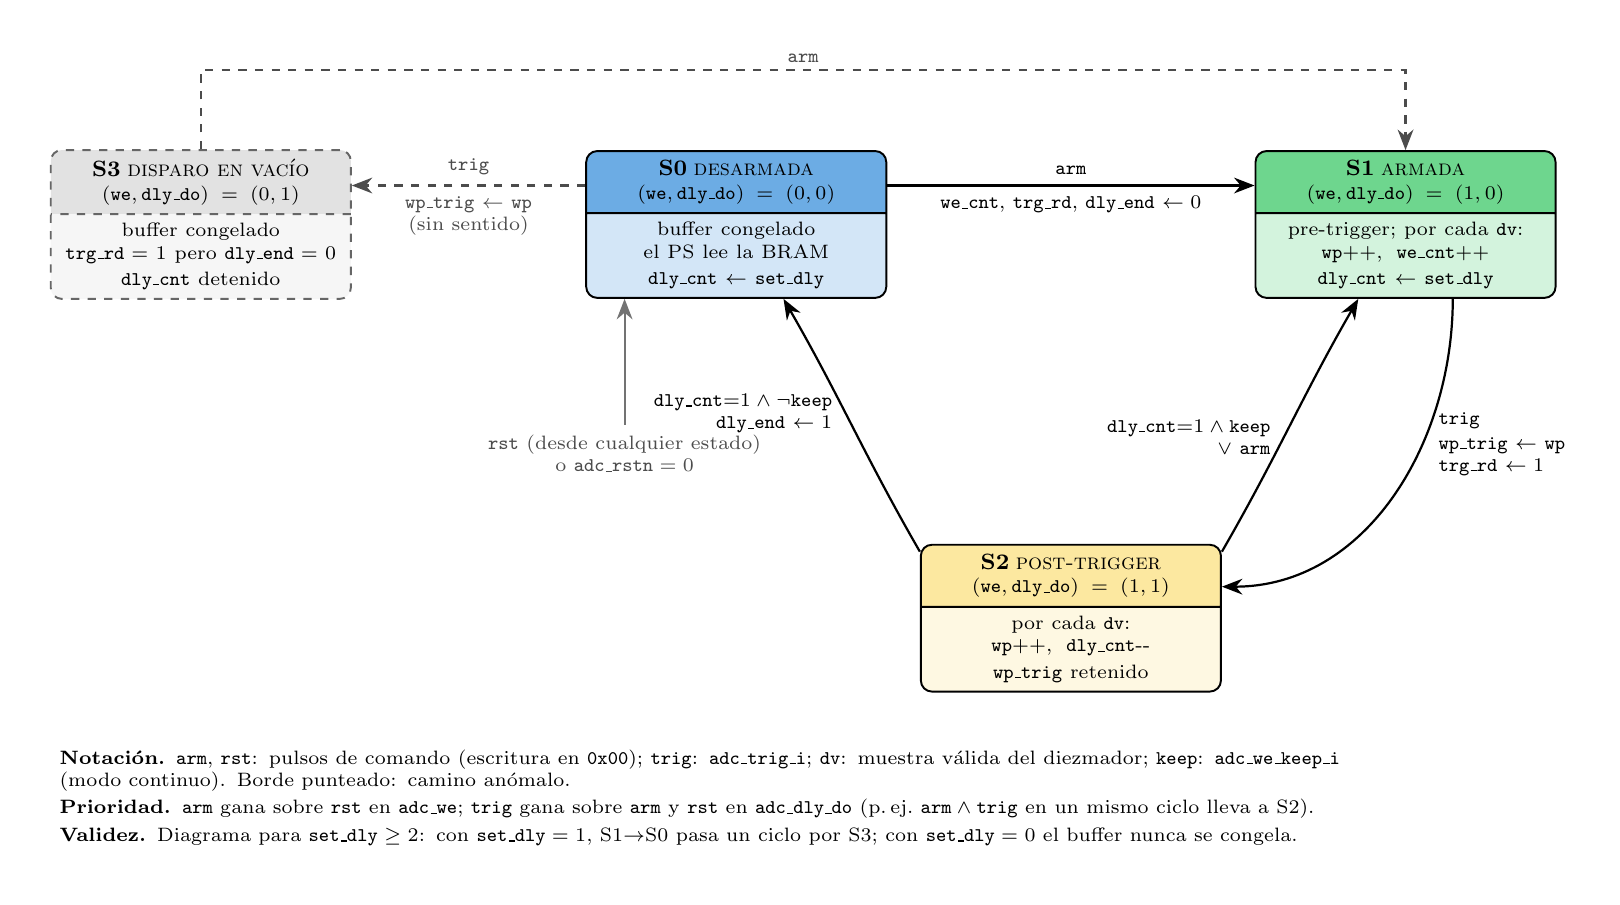
\begin{tikzpicture}[node distance=2cm, show background rectangle, inner frame sep=8pt,
  background rectangle/.style={fill=white, draw=none}]

% ===================================================================== estados
\node[estado=azul] (S0) at (0,0) {
  \cab{S0}{desarmada}{0,0}
  \nodepart{two}\scriptsize buffer congelado\\
  el PS lee la BRAM\\
  \s{dly\_cnt} $\leftarrow$ \s{set\_dly}
};

\node[estado=verde] (S1) at (8.5,0) {
  \cab{S1}{armada}{1,0}
  \nodepart{two}\scriptsize pre-trigger; por cada \s{dv}:\\
  \s{wp}{+}{+},\; \s{we\_cnt}{+}{+}\\
  \s{dly\_cnt} $\leftarrow$ \s{set\_dly}
};

\node[estado=amarillo] (S2) at (4.25,-5) {
  \cab{S2}{post-trigger}{1,1}
  \nodepart{two}\scriptsize por cada \s{dv}:\\
  \s{wp}{+}{+},\; \s{dly\_cnt}{-}{-}\\
  \s{wp\_trig} retenido
};

\node[anomalo] (S3) at (-6.8,0) {
  \cab{S3}{disparo en vacío}{0,1}
  \nodepart{two}\scriptsize buffer congelado\\
  \s{trg\_rd}${}=1$ pero \s{dly\_end}${}=0$\\
  \s{dly\_cnt} detenido
};

% ============================================================ reset global ===
\coordinate (rst) at ($(S0.south west)+(0.5,-1.6)$);
\draw[global] (rst) node[below, font=\scriptsize, align=center, black!70]
  {\s{rst} (desde cualquier estado)\\ o \s{adc\_rstn}${}=0$}
  -- (rst |- S0.south);

% ============================================================ transiciones ===
% S0 -> S1 : armar
\draw[trans] (S0.text split east |- S0.north east) ++(0,-0.45) coordinate (a0)
  (a0) -- (a0 -| S1.west)
  node[guarda, midway, above=2pt, fill=none] {\s{arm}}
  node[guarda, midway, below=2pt, fill=none]
  {\s{we\_cnt}, \s{trg\_rd}, \s{dly\_end} $\leftarrow 0$};

% S1 -> S2 : trigger
\draw[trans] ([xshift=6mm]S1.south) to[out=-90, in=0]
  node[guarda, pos=0.35, right=4pt, fill=none, align=left]
  {\s{trig}\\[1pt] \s{wp\_trig} $\leftarrow$ \s{wp}\\ \s{trg\_rd} $\leftarrow 1$}
  ([yshift=4mm]S2.east);

% S2 -> S1 : modo continuo o re-armado
\draw[trans] ([yshift=-1mm]S2.north east) to[out=60, in=-120]
  node[guarda, pos=0.45, left=3pt, fill=none, align=right]
  {$\s{dly\_cnt}{=}1 \wedge \s{keep}$\\ $\vee\ \s{arm}$}
  ([xshift=-6mm]S1.south);

% S2 -> S0 : fin del post-trigger, congela
\draw[trans] ([yshift=-1mm]S2.north west) to[out=120, in=-60]
  node[guarda, pos=0.55, left=3pt, fill=none, align=right]
  {$\s{dly\_cnt}{=}1 \wedge \neg\s{keep}$\\ \s{dly\_end} $\leftarrow 1$}
  ([xshift=6mm]S0.south);

% S0 -> S3 : trigger con la FSM desarmada
\draw[trans, dashed, black!70] (a0 -| S0.west) -- (a0 -| S3.east)
  node[guarda, midway, above=2pt, fill=none] {\s{trig}}
  node[guarda, midway, below=2pt, fill=none, align=center]
  {\s{wp\_trig} $\leftarrow$ \s{wp}\\ (sin sentido)};

% S3 -> S1 : armar (el disparo ya se consumió)
\draw[trans, dashed, black!70] (S3.north) -- ++(0,1.0) coordinate (t3) -| (S1.north)
  node[guarda, pos=0.25, above=1pt, fill=none] {\s{arm}};

% ================================================================= leyenda ===
\node[font=\scriptsize, align=left, anchor=north west, text width=16.5cm]
  at ($(S3.west |- S2.south)+(0,-0.6)$) {%
  \textbf{Notación.} \s{arm}, \s{rst}: pulsos de comando (escritura en \s{0x00});
  \s{trig}: \s{adc\_trig\_i}; \s{dv}: muestra válida del diezmador;
  \s{keep}: \s{adc\_we\_keep\_i} (modo continuo). Borde punteado: camino anómalo.\\[2pt]
  \textbf{Prioridad.} \s{arm} gana sobre \s{rst} en \s{adc\_we};
  \s{trig} gana sobre \s{arm} y \s{rst} en \s{adc\_dly\_do}
  (p.\,ej.\ \s{arm}${}\wedge{}$\s{trig} en un mismo ciclo lleva a S2).\\[2pt]
  \textbf{Validez.} Diagrama para \s{set\_dly}${}\ge 2$: con \s{set\_dly}${}=1$,
  S1$\to$S0 pasa un ciclo por S3; con \s{set\_dly}${}=0$ el buffer nunca se congela.%
};

\end{tikzpicture}
\end{document}
